\documentclass[acmtog]{acmart}

% remove the stuff template info we don't want
\settopmatter{printacmref=false}
\renewcommand\footnotetextcopyrightpermission[1]{}
\pagestyle{plain}

\makeatletter
\renewcommand\@formatdoi[1]{\ignorespaces}
\makeatother

\authorsaddresses{}
\acmDOI{}

\fancyfoot{}
%

\usepackage{booktabs} % For formal tables
\usepackage{graphicx}
\usepackage[export]{adjustbox}
\usepackage{float}
\usepackage{natbib}

% TOG prefers author-name bib system with square brackets
\citestyle{acmauthoryear}
\setcitestyle{numbers}

\usepackage[ruled]{algorithm2e} % For algorithms
\renewcommand{\algorithmcfname}{ALGORITHM}

\SetAlFnt{\small}
\SetAlCapFnt{\small}
\SetAlCapNameFnt{\small}
\SetAlCapHSkip{0pt}
\IncMargin{-\parindent}

\begin{document}

\title{Automated Playlist Generation}

\author{Kade Keith}
\affiliation{ \institution{Stanford University} }
\email{kade@stanford.edu}
\author{Demetrios Fassois}
\affiliation{ \institution{Stanford University} }
\email{dimifass@stanford.edu}

\begin{abstract}
Our project explores generating music playlists based on a song or set of seed songs using diverse features ranging from lyrical sentiment to song popularity. We approach the problem as both a graph problem and as a classification problem, and evaluate our results based on real human-curated playlists. We find that our feature set and models perform the task well and that lyrical content in particular is a good indicator for playlist generation.
\end{abstract}

\maketitle
\thispagestyle{empty}

\section{Introduction}

With the growth of music streaming services, there are now more songs than ever at music listeners fingertips. Because of this growth, the art of constructing playlists has become increasingly challenging, and discovering new music in the expanse of choices is a daunting task. For this reason, we explore methods of automatic playlist generation that can take a few songs as a seed set and generate a complete playlist for the listener. We explore this as both a classification problem, in which one part of the playlist is the train data and the reminder the test, and as a  generative graph search problem in which we want to recommend similar songs to the provided seeds.

\section{Related work}

Playlist generation, and the problem of music recommendation and discovery more generally, is a broad problem that has been attempted with many different approaches. Geoffray Bonnin and Dietmar Jannach \cite{Bonnin2013ACO} provide an overview of these approaches and evaluation methods. They provide an overview of simple approaches to the problem: neighborhood approaches (k-nearest-neighbors), transition probability approaches (markov chains), and popularity-based approaches (same artist's greatest hits, similar artists greatest hits).

Related to the neighborhood approach listed before, Beth Logan \cite{BethLogan} at Hewlett-Packard labs provides an overview of considering a playlist as a trajectory through a graph. When considering songs as a graph, defining a distance function is of primary importance, which Logan and Ariel Salomon \cite{LoganSalomon} have also worked on. Masoud Alghoniemy and Ahmed H. Tewfik \cite{Alghoniemy01anetwork} explore songs as a network in which playlists can be found using a network-flow model.

Digging deeper into the importance of song order in playlists, Maillet et. al. \cite{Maillet09steerableplaylist} extract pairs of songs from playlists and learn transition probabilities specifically from how often that exact pair of songs shows up in sequence. Ragno, R. and Burges, C. J. C. and Herley, C. \cite{Ragno:2005:ISM:1101826.1101840} combine the previously mentioned approaches to represent songs in a graph where the edge weights are determined by how frequently the two songs appear next to each other in the training data.

\section{Dataset and Features}

We combine data from a number of sources in our project. The primary source is the Million Song Dataset (MSD) \cite{msd}, and the corresponding lyrics dataset, which provides lyrics for roughly a quarter of those songs in a bag-of-words format. We then augment that info with audio features and popularity info from Spotify \cite{spotify}.

We started with just under half of the Million Song dataset. The dataset in it's entirety is almost 30 GB large, so we cut it down to make processing it faster. After filtering out songs without lyrics and songs for which we could not fetch info on from Spotify, we ended up with a final dataset of 76,442 songs. Enumerated below are the features.
\\
\begin{center} \textbf{Raw features} \end{center}
\begin{tabular}{lll}
Year              & MSD, Spotify    \\
Tempo             & MSD, Spotify    \\
Timbre            & MSD             \\
Danceability      & MSD, Spotify    \\
Energy            & MSD, Spotify    \\
Loudness          & Spotify         \\
Popularity        & Spotify         \\
Speechiness       & Spotify         \\
Acousticness      & Spotify         \\
Instrumentalness  & Spotify         \\
Liveness          & Spotify         \\
Valence           & Spotify         \\
\end{tabular}
\\\\
We crafted 3 additional features using the modeling techniques described in the next section.
\begin{center} \textbf{Derived features} \end{center}
\begin{tabular}{lll}
Sentiment             & Naive Bayes on Lyrics   \\
Lyrics Category       & LDA on Lyrics           \\
Timbre Hidden Value   & HMM on Timbre           \\
\end{tabular}
\\
\begin{center} \textbf{Example song} \end{center}
\begin{verbatim}
artist_name                       Western Addiction
audio_features                 {
                                 `Tempo' : 120,
                                 `Energy' : 0.65,
                                 `Loudness' : 0.44,
                                 ...
                                 `Valence' : 0.38,
                               }
popularity                                     0.11
segments_timbre         [
                         [0.0, 171.13, 9.469, ...],
                         [0.089, -30.06, ...],
                         ...
                         [24.937, 37.465, ...]
                        ]
sentiment_score                                   1
song_id                          SOQPWCR12A6D4FB2A3
title              A Poor Recipe For Civic Cohesion
track_id                         TRAAAAV128F421A322
year                                           2005
song_artist_title    western addiction, a poor r...
lda_probs_topic_1                          0.215142
lda_probs_topic_2                          0.774669
lda_probs_topic_3                         0.0101883
hidden_path_avg                            0.203233
\end{verbatim}
The overall flow we used to process this data was: 1) Remove extraneous fields and songs with incomplete data from dataset 2) Collect and merge Spotify features via their API 3) Run Naive Bayes and Latent Dirichlet Allocation on lyrics and merge in those features 4) Run Hidden Markov Model on Timbre and merge in resulting feature.

As for our training playlists we also used Spotify as the source. We wrote a script to collect top search results of playlists for whatever terms we provided, and ran that for popular playlist terms like ``summer'', ``love'', ``break up'', and ``workout.'' In the end we gathered over 300 playlists. For training our models we filtered to only playlists for which we recognized a significant number of their songs. In the end that gave us a set of around 40 possible playlists of varying lengths and genres. In general there was a bias toward Rock playlists, and that is the most prominent genre in the Million Song Dataset.

\subsection{Feature Extraction}
\subsubsection{Latent Dirichlet Allocation}

We chose all playlists for which we had an overlap of at least 30 songs with our dataset. We then tokenized and removed all stop words from the lyrics of the songs from every playlist, in order for the playlists to be treated as documents and the lyrics as words in the Latent Dirichlet allocation model. Latent Dirichlet allocation is a generative statistical model which posits that the lyrics from every playlist can be explained by a fixed number of unobserved topics, which would help explain some similarity between playlists. In our case, we chose the number of common topics to be 3, and the process that the generative model describes is the following: \newline
For the $M$ playlists, each of length $N_{i}$ we have the following parameters and distributions:
\begin{enumerate}
  \item Probability $\theta_{i} \sim Dir(\alpha)$, where $Dir(\alpha)$ is a Dirichlet distribution with parameter $\alpha$ and $i \in {1, ..., M}$
  \item Probability $\phi_{k} \sim Dir(\beta)$, where $k \in {1,2,3}$ is the index of the topic.
  \item For each word in the lyrics from all playlists, for $i, j$, where $i \in {1, ..., M}$ and $j \in {1, ..., N_{i}}$:
     \begin{enumerate}
       \item Chose a topic $z_{i, j} \sim Multinomial(\theta_{i})$
       \item Chose a word $w_{i, j} \sim Multinomial(z_{i, j})$
     \end{enumerate}
\end{enumerate}

The probabilities that were output from the model for each of the three topics for each song were subsequently used as features by the final model.

% Numbered Equation
\begin{equation}
\label{eqn:01}
P(t)=\frac{b^{\frac{t+1}{T+1}}-b^{\frac{t}{T+1}}}{b-1},
\end{equation}
where $t=0,{\ldots}\,,T$, and $b$ is a number greater than $1$.

\subsubsection{Hidden Markov Model on timbre segments}

Timbre is defined as the perceived sound quality of a musical note, sound or tone. The MSD dataset contains the time sequence of the timbre feature as a vector of 12 unbounded values centered around 0. These values represent different characteristics of the spectral
surface, ordered by degree of importance. For example, the first dimension represents the average
loudness of the segment, the second one describes brightness, the third one describes the flatness of a sound, the fourth describes sounds with a stronger attack etc. We averaged the vector features for every time segment for each song, in order to have a time series of the actual timbre of each segment.
We subsequently trained a hidden Markov model on the timbre sequence of a random sample of 5,000 songs. The model was fit using the EM algorithm which is a gradient-based optimization method and can therefore get stuck in local optima. For this reason we fit the model with various initializations and selected the highest scoring one.
The inferred optimal hidden states of the timbre segments of all songs were predicted by the model, employing the Viterbi algorithm.
For each song the optimal hidden states were averaged to provide a single description of the path followed, which was used as an additional feature by the final models.
For the training data the average value of the timbre which had a hidden value of 1 was 4.96, for hidden value of 1 they had an average value of the timbre of 13.76 and for a hidden value of 2 an average of -5.35.

\subsubsection{Sentiment analysis}

Although it ended up not being particularly useful in the end (see the feature importance in a later section), we pursued extracting sentiment from lyrics as our baseline analysis.
\[
  p(C_k | x) = \frac{P(C_k)P(x | C_k)}{p(x)}
\]
We used Naive Bayes (with the NLTK movie review corpus as training data \cite{nltk}) to score each song as either positive or negative.

\section{Methods}
\label{sec:sim}

Two different methodologies were pursued. In the first, we tried different classification algorithms both for a single playlist prediction and multi-class prediction for 26 playlists. In the second, we used graph-based approaches to predict songs and measure the similarity between our predicted songs and the actual songs.

\subsection{Classification}

We first applied binary classification using a single playlist ('60s, 70s, 80s Classic Rock') as the target and randomly selecting songs that didn't belong to it as well. The training set consisted of 98 songs, while the test set included 34 songs. After standardizing the features we performed grid search on the hyper-parameters for a logistic regression and support vector machine classifier. For logistic regression the regularization strength was fine tuned employing 10-fold cross-validation, while for the support vector classifier the regularization was also optimized using grid search. The other parameters that were chosen during cross validation were the kernel (linear or exponential). For the exponential kernel $e^{-\gamma {\Vert x -x' \Vert}^{2}}$ the $\gamma$ parameter was also optimized. \cite{PythonMachineLearning}

\subsection{Graph Models}

\subsubsection{K-nearest neighbors}
The simplest graph approach is k nearest neighbors. We represent each song as a point in n-dimensional space according to our normalized features. Then we select the next songs for that playlist based on proximity to the average (centroid) of all of the seed songs.

\subsubsection{K-shortest path}

Another way to think about a playlists is as a path through a graph. Given two songs, we construct a playlist as the shortest path of length k between them. This is particularly intriguing if the two seed songs are very different.

With this approach we have to be careful as the runtime grows exponentially. Via dynamic programming, the shortest path to node v of length k is:
\[
  short\_path[v][k] = \min_u \Big ( short\_path[u][k-1] + distance[u][v] \Big)
\]
Thus the algorithm is just to iterate from $0..k$ filling in the $short\_path$ for all $v$ and taking care to avoid cycles.

This runs in $O(kV^2)$ time where $V$ is the number of songs. The runtime can be further optimized by restricting the search space to only include songs in the ``neighborhood'' of the two seeds. We do this by finding their average and excluding songs that lay too far away from that centroid. In our case we use half the distance between the songs plus some constant. Thinking about this geometrically, if the data was in two dimensions then the neighborhood would be all songs within a circle where the two seeds lie opposite each other on the edge of the circle. While this effectively reduces the graph if the songs are near one another, if the songs are very different then the neighborhood is larger. Thus the runtime grows exponentially by a factor of how different the seeds are. This proved to be problematic in case where the neighborhood was extremely large, as the algorithm was painfully slow if the neighborhood was larger than around 4000 songs.

\section{Results}

Results for the two main methodologies followed are presented below.

\subsection{Classification}
The logistic regression model achieved training accuracy of 95.9\% and CV accuracy of 94.8\%. The SVC outperformed the logistic regression model, with the best model achieving training accuracy of 96.9\% and CV accuracy of 95.9\%. The best model's parameters used a linear kernel with regularization. The final test accuracy for the SVC was 94.1\%.
The learning curve for the SVM model is presented below in figure \ref{fig:learning_curve} and it shows that it generalizes well over unseen data.
\newline

The validation curve for the SVC model can be seen below in figure \ref{fig:validation_curve}, which justifies how the particular value for the regularization hyper-parameter was chosen. The cross-validation accuracy decreases as the regularization parameter C increases even though the training accuracy keeps increasing, which would indicate overfitting.

The confusion matrix for the SVC model on the test data can also be seen below in figure \ref{fig:confusion_matrix}.

The ROC curve is also plotted below in figure \ref{fig:ROC_curve} which shows an excellent area under the curve.

%figure
\begin{figure}[h]
  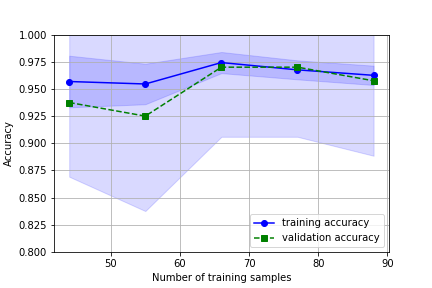
\includegraphics[width=0.5\textwidth]{learning_curve}
  \caption{Learning curve for SVC}
  \label{fig:learning_curve}
\end{figure}

%figure
\begin{figure}[h]
  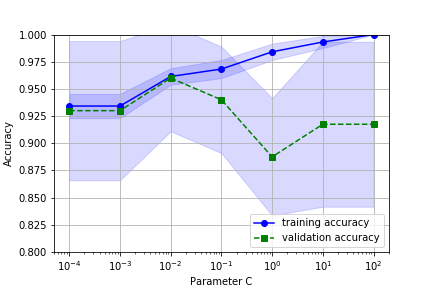
\includegraphics[width=0.5\textwidth]{validation_curve}
  \caption{Validation curve for SVC}
  \label{fig:validation_curve}
\end{figure}

%figure
\begin{figure}[h]
  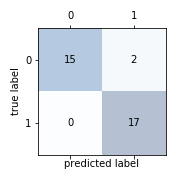
\includegraphics[width=0.33\textwidth]{confusion_matrix}
  \caption{Confusion matrix for SVC}
  \label{fig:confusion_matrix}
\end{figure}

%figure
\begin{figure}[h]
  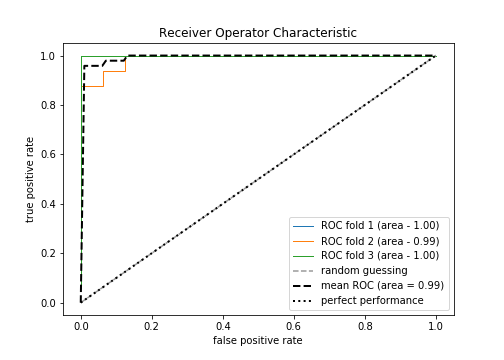
\includegraphics[width=0.5\textwidth]{ROC_curve}
  \caption{ROC curve for SVC}
  \label{fig:ROC_curve}
\end{figure}

% Table
\begin{table}%
\caption{SVC performance on single playlist}
\label{tab:one}
\begin{minipage}{\columnwidth}
\begin{center}
\begin{tabular}{ll}
  \toprule
  Test accuracy    & 94.1\%\\
  Recall  & 100\%\\
  Precision    & 88.2\%\\
  F1-score    & 93.7\%\\
  \bottomrule
\end{tabular}
\end{center}
\bigskip\centering
\footnotesize
 \emph{Precision scores for SVC model}
\end{minipage}
\end{table}%

We also applied multi-class classification for 9 playlists for which we had more than 50 songs in our dataset. With this modeling technique called one-vs-all classification, one classifier is fitted for each class against all of the other classes. The training set consisted of 718 songs, while the test set included 180 songs. Given the superior performance of the SVC model on one playlist, we optimized it in the multi-class setting using grid search and cross-validation. The grid search for the multi-class SVC yielded a model with training accuracy of 64.5\% and CV accuracy of 54.7\%. Grid search with cross-validation was also performed on a random forest model in order to estimate the number of trees in the forest, the number of features to consider for the best split, the maximum depth of a tree, the minimum number of samples required to split an internal node, the minimum number of samples required for a leaf node, whether bootstrap samples are used and what criterion between Gini impurity and entropy is used for a split. The best random forest model achieved a training accuracy of 68.4\% and cross-validated accuracy of 56.4\%. The test accuracy was 52.2\%. The feature importance from the random forest in order of usefulness can be seen in the plot below. Importance is calculated for each feature from the amount that each split improves the performance criterion, weighted by the number of observations of the node.

%figure
\begin{figure}[h]
  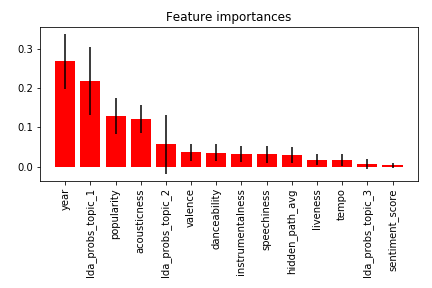
\includegraphics[width=0.5\textwidth]{feature_importance2.png}
  \caption{Figure: Feature importance of random forest for multi-class prediction}
  \label{fig:ROC_curve}
\end{figure}

We also applied another technique, employing a random forest classifier and encoding each tree as a feature index in a new high-dimensional feature space. Then we applied a logistic regression model on this sparse, one-hot encoded embedding of the data. The test set accuracy achieved with this method was 51.1\%.
The final technique that was employed was an ensemble method, namely plurality voting, which selects the playlist that received the most votes from the majority of a group of classifiers. The classifiers we implemented for plurality voting were logistic regression, SVC, decision tree, random forest and KNN. The cross-validated accuracy of the plurality voting ensemble was 55\% $\pm$ 2\%. The classifiers' cross-validated accuracy is summarized in table \ref{tab:two}.
% Table
\begin{table}%
\caption{Cross-validated accuracy of classifiers in plurality voting}
\label{tab:two}
\begin{minipage}{\columnwidth}
\begin{center}
\begin{tabular}{ll}
  \toprule
  Logistic Regression    & $51\% \pm 3\%$\\
  SVC  & $49\% \pm 3\%$\\
  Decision Tree  & $46\% \pm 3\%$\\
  Random Forest  & $55\% \pm 2\%$\\
  KNN  & $48\% \pm 2\%$\\
  Plurality Voting  & $55\% \pm 2\%$\\
  \bottomrule
\end{tabular}
\end{center}
\bigskip\centering
\footnotesize
 \emph{Plurality voting CV performance}
\end{minipage}
\end{table}%

\subsection{Graph Models}

For our graph approaches we report a number of distances. In each case the distances have been normalized so that the maximum possible distance between any two songs would be 1. These results are averaged over
40 playlists in the case of k-nearest-neighbors, and 20 playlists in the shortest-path approach (some playlists were excluded for performance reasons). For knn each playlist was split it 75/25 into train/test data. For the shortest path, two songs were selected arbitrarily and the shortest path the length of the playlist was chosen between them.

As a baseline we report the average distance within the training playlist. Then we report the average distance from our k-nearest-neighbors predictions to the positive train data (the seed songs), followed by the average distance to the positive test data (the remaining songs on the playlist). We then report the distance to the negative test set (a random selection songs). Finally, we report the average distance of our path generated by the shortest path search to the actual playlist. \\

\begin{center}
\begin{tabular}{ll}
  \toprule
  Within playlist                      & 0.241 \\
  (KNN) Prediction to train songs      & 0.191 \\
  (KNN) Prediction to test songs       & 0.196 \\
  (KNN) Prediction to random songs     & 0.292 \\
  (Path) Prediction to actual playlist & 0.231 \\
  \bottomrule
\end{tabular}
\\
\footnotesize
  \emph{Average Distances}
\end{center}

For these results, the primary thing we hope is that the distance from the predicted songs to the test data will be small and comparable to the distance from the predicted songs to the test data to validate that the predictions are similar to the seed. This is what we see. One initially surprising thing is that the distance within the playlist is higher than the distance of the predictions to both the train and test data. This is because the playlist cannot overlap with itself, whereas the prediction may contain the actual songs on the playlists. They will have a distance of zero with themselves which brings the average down.

\section{Conclusions and Future Work}

We are pleased with how both approaches to the task performed, and we attribute the accuracy to the strength of our features, both raw and derived. In particular we were pleased to see the importance of lyrics when making playlists proven, as that was one of our initial hypotheses. When making a playlist, people choose songs that make them feel a certain way, and lyrics are huge part of that. People also choose songs that they've actually heard of, so popularity is important.

Future general improvements could focus on leveraging more song characteristics and also deriving more crafted features from them in order to improve performance of the final models. This would be supported by more data gathering, in particular of genres like Hip-Hop which are underrepresented in the MSD.

Additionally we think it would be quite interesting to compare the learned parameters of our various models between playlists. This way we can examine what kind of differences there are in what motivates individuals when they make playlists.


\section{Contributions}
Kade was responsible for the initial pre-processing and gathering of the dataset and the graph models. He implemented the sentiment analysis portion of feature extraction and the baseline regression classification. He was the primary author on the various reports. He made the poster and gave the recorded the poster presentation.

Demetrios wrote the script to augment the MSD data with Spotify features. He did the work on LDA and HMM to extract features from Lyrics and Timbre. He tested a number of different classification models and built the cross validation pipeline for choosing and evaluating the best model. This included generating the reported figures and reporting feature importance.

% Bibliography
\bibliographystyle{plain}
\bibliography{lit}{}

%\input{samplebody-journals}

\end{document}
